\documentclass{article}
\usepackage{geometry}
 \geometry{
 a4paper,
 left=30mm,
 right=30mm,
 top=30mm,
 bottom=30mm,
 }
 
\usepackage[footnotes,definitionLists,hashEnumerators,smartEllipses,hybrid]{markdown}
\usepackage[utf8]{inputenc}
\usepackage[document]{ragged2e} % remove line justify
\usepackage{dblfloatfix}
\usepackage{microtype}
\usepackage[none]{hyphenat}
 \usepackage{setspace}
	%\setstretch{1.2} %SOPHIA 


\usepackage{fontspec}
\defaultfontfeatures{Mapping=tex-text,Scale=MatchLowercase} %SOPHIA
\setmainfont{Source Sans Pro--Light
}[BoldFont={Source Sans Pro-Regular},
 ItalicFont={Source Sans Pro-Light Italic},
 ] %SOPHIA
 
\usepackage{xcolor}
\definecolor{sophiablue}{HTML}{0A2E4A}
\definecolor{sophiapink}{HTML}{E32A5C}
 \color{sophiablue} %SOPHIA
 
\usepackage{authblk} % authors

\usepackage{lineno} % used along with \linenumbers after begin document. 
\usepackage{setspace} % line spacing
  \setstretch{1.4}
\usepackage{enumitem}
\setlist[itemize]{noitemsep}

\usepackage{microtype} % Creates better spaced text
\usepackage{siunitx} % SI units 

\usepackage{xcolor} % Setting colours and their usage
  \definecolor{natureblue}{RGB}{5,110,210}

\usepackage[colorlinks]{hyperref} % Colour for hyperlinks, (URLs, citations, cross reference)
  \AtBeginDocument{%this allows colours to change from the defined article template.
  \hypersetup{
  linkcolor={sophiapink},
  citecolor={sophiapink},
  filecolor=blue!50!black,
  urlcolor=sophiapink,
  }}

\usepackage{natbib}
  \setcitestyle{square,numbers,sort&compress}
  \setcitestyle{sort&compress}
\usepackage{hypernat} % hypernat also required to allow citations to compress. 
\usepackage{graphicx}
\graphicspath{ {images/} } % sets the path to image files (Figures)

\usepackage{booktabs} % required for tables
\usepackage{rotating,tabularx} % tabularx is the table style used, rotating can also be used
\usepackage{longtable}
\newcolumntype{Z}{ >{\centering\arraybackslash}X } % defining table content layout per box
\usepackage{ltablex} % allow page break between lines in tabularx
\usepackage{caption} \captionsetup{font=normalsize} % to set the caption size as normal even when table is tiny.

\usepackage{pdflscape} % for rotated table
\usepackage{multirow} % for table

\begin{document}
\date{} %don't want date printed
%make title bold and 14 pt font (Latex default is non-bold, 16 pt)
\title{\Large \bf Comparison of two target sequencing approaches.
\footnote{This document's source code is available from the 
\href{https://github.com/DylanLawless/kit_assess/blob/master/latex/report.tex}{GitHub repository}.
All code used in this report is available on the 
\href{https://github.com/DylanLawless/kit_assess}{GitHub repository}.}
}
%\thanks {Use thanks if u you need it}
%for single author (just remove % characters)

\author[1]{\rm Dylan Lawless, PHD}
\affil[1]{Global Health Institute, School of Life Sciences, École Polytechnique Fédérale de Lausanne, Switzerland, 
\color{sophiapink}{Dylan.Lawless@epfl.ch}
}
%\affil[ ]{\textit {\{email1,email2,email3,email4\}@xyz.edu}}
\maketitle
%\linenumbers

%\cite{•}

\section{Introduction}
\label{intro}
The two datasets (AH S1 and CH S2) of paired-end short reads were generated from the same human DNA NGS library for clinical diagnosis of solid tumor. 
They were obtained through two different target sequencing approaches with corresponding target region file provided (hg19). 
Herein, we evaluate their performances for use in clinical diagnose.

\section{Details for technical writing report}
\textit{Note:}
This section contains the main information required for a technical report.
The remainder of this document contains additional information which is \textit{not} required for further reports, and includes duplicate references to files listed here.
Please include:

\begin{itemize}
\item \textbf{Introduction}: all details from sec. \ref{intro}.
\item \textbf{Data source}: all details from sec. \ref{data_source}.
\item \textbf{Protocol details}: a hyperlink to the protocol source: [\href{https://github.com/DylanLawless/kit_assess/README.md}{link}].
\item \textbf{Result}: Result summary sec. \ref{result_summary}.
\item \textbf{Figures}: \ref{fig:p1}, \ref{fig:qualimap_map_qual_hist},  and \ref{fig:qualimap_gen_cov_ref}.
\item \textbf{Conclusion}: all details from sec \ref{conclusion}.
\end{itemize}

\section{Methods}
\subsection{Data source}
 \label{data_source}

\begin{itemize}
\item \textbf{Description}: The sequencing group performed library preparation for two (2) samples (AH and CH) using \href{https://www.sophiagenetics.com/clinical/oncology/solid-tumors/}{Kit X}.
The performance of each was assessed with several bioinformatic methods including read quality control and performance when aligning to reference genome
[\href{https://github.com/DylanLawless/kit_assess}{code available here}].
\item \textbf{Data source}: raw sequence data was received from
 [\href{https://www.sophiagenetics.com}{link group and contact address}].
\item \textbf{Date}: 2022-02-14
\item \textbf{Link to tickets where submission was logged}: [\href{https://www.sophiagenetics.com}{link}]
\item \textbf{Data integrity}: [\href{https://github.com/DylanLawless/kit_assess/blob/master/src/raw.md5sum}{link metadata md5sum}].
\end{itemize}

\subsection{Configuration}

Local env: macOS v11.6 \href{https://support.apple.com/macos}{software},
Remote env: Red Hat Enterprise Linux Server 7.6 (Maipo)  \href{https://www.redhat.com/en/technologies/linux-platforms/enterprise-linux}{software},
compiler intel: (19.0.5 and 19.1.1),
\href{https://www.intel.com/content/www/us/en/developer/tools/oneapi/commercial-base-hpc.html#gs.ppyt3x}{software},
R: R v4.1.0 Camp Pontanezen  \href{https://www.r-project.org}{software},
R libraries: versions unlisted,
fastqc: v0.11.7 \href{https://www.bioinformatics.babraham.ac.uk/projects/fastqc/}{software},
samtools: v1.10 \href{https://www.htslib.org}{software},
bwa: v0.7.17 \href{https://janis.readthedocs.io/en/latest/tools/bioinformatics/bwa/bwamem.html}{software},
picard: v2.20.8  \href{http://broadinstitute.github.io/picard/}{software}.
qualimap v2.2.1 \href{http://qualimap.conesalab.org}{qualimap}.

\subsection{Analysis code}
All code available at \href{https://github.com/DylanLawless/kit_assess}{link: GitHub/kit\_assess}. 

Protocol order:
\begin{itemize}
\item src/md5sum.ch
\item src/read\_count.sh
\item fastQC: manual run all fastq and save to ./processed/fastqc
\item fastqcr: Assess fastqc rerpots further
\item src/target\_info.sh
\item src/1.trim.sh
\item src/2.align.sh
\item src/3.sort.sh
\item src/mapping.sh
\end{itemize}

\section{Results}
Data for this report can be found on \href{https://github.com/DylanLawless/kit_assess}{link: GitHub/kit\_assess}. 
Analysis results are separated into QC of fastq data (sec. \ref{fastq_data}), QC after alignment to reference genome GRCh37 (sec. \ref{align_data}), and exploration of target coding regions 
(sec. \ref{coding}).

\subsection{Result summary}
\label{result_summary}

Based on 
[1] QC of fastq data,
[2] QC after alignment to reference genome GRCh37, and 
[3] exploration of target coding regions,
AH S1 performed better than CH S2 for use in clinical diagnosis of solid tumor.
The read depth and uniform coverage provided for AH S1 outperformed CH S2 and is beneficial in tumor sequencing for calling germline variants, somatic variants, CNV or structural changes.

\subsection{Fastq data}
\label{fastq_data}
To assess the qulity of fastq data, \href{https://www.bioinformatics.babraham.ac.uk/projects/fastqc/}{FastQC} was used. 
Full html reports for each file are linked:
\begin{itemize}
	\item \href{https://lawlessgenomics.com/pages/sophia/AH_S1_L001_R1_fastqc.html}{AH\_S1\_L001\_R1\_fastqc}
	\item \href{https://lawlessgenomics.com/pages/sophia/AH_S1_L001_R2_fastqc.html}{AH\_S1\_L001\_R2\_fastqc}
	\item \href{https://lawlessgenomics.com/pages/sophia/CH_S2_L001_R1_fastqc.html}{CH\_S2\_L001\_R1\_fastqc}
	\item \href{https://lawlessgenomics.com/pages/sophia/CH_S2_L001_R2_fastqc.html}{CH\_S2\_L001\_R2\_fastqc}
\end{itemize}

The results of fastQC were also assessed by use of \href{https://rpkgs.datanovia.com/fastqcr/index.html}{fastqcr}.
The full html report is linked:
\begin{itemize}
	\item \href{https://lawlessgenomics.com/pages/sophia/qc_report.html}{Report assessment of fastQC}
\end{itemize}

\begin{enumerate}
\item Total sequences or the number of reads for each samples: 1000000
\item Per base sequence quality: \textbf{All samples performed sufficiently}. Summarised in Figure \ref{fig:p1}
	\begin{itemize}
	\item Median value (red line):
		 \textbf{AH good quality} (qual >28),
		 \textbf{CH good quality }(qual >28).

	\item Inter-quartile range (25-75\%) (yellow box): 
		 \textbf{AH good quality} (qual >28),
		\textbf{ CH medium to good quality}  (qual >20).

	\item Upper and lower 10\% and 90\% whiskers points:
		 \textbf{AH medium to good quality} (qual >28),
		 \textbf{CH poor to good quality} (qual >14).
	
	\item Mean quality (blue line):
		\textbf{AH good quality} (qual >28),
		\textbf{CH medium to good quality}  (qual >20).
	\end{itemize}

\item Per tile sequence quality: \textbf{All samples performed sufficiently}. No warning.
\item Per sequence quality score: \textbf{All samples performed sufficiently},  summarised in Figure \ref{fig:p2}.
\item Per base sequence content. \textbf{All samples flagged} with warning indicating 
a difference greater than 10\% in any position. However, this is potentially due targeted capturing, Figure \ref{fig:p3}.

\item Per sequence GC content. \textbf{All samples failed} based on modal GC content as calculated from the observed data and used to build a reference distribution. The sum of the deviations from the normal distribution represents more than 30\% of the reads.
However, the sharp peaks (as seen on AH [Top]) are most likely due to enriched duplicate sequences from targeted capturing and do not necessarily indicate poor quality, Figure \ref{fig:p4}.

\item Sequence Length Distribution:\textbf{ AH reads were all 150}, while \textbf{CH reads were 35-151}.
 
\item Sequence Duplication Levels: Percentage of duplicate reads were \textbf{AH 96.01\%-96.55\%} and \textbf{CH 65.44\%-67.13}\%. Figure \ref{fig:p5}

\item Adapter Content: Figure \ref{fig:p6},
	\textbf{AH Illumina Universal adaptor} and
	\textbf{CH Adaptor not detected}.
\end{enumerate}

\begin{figure}[h] \hspace*{0cm} 
\begin{center}
    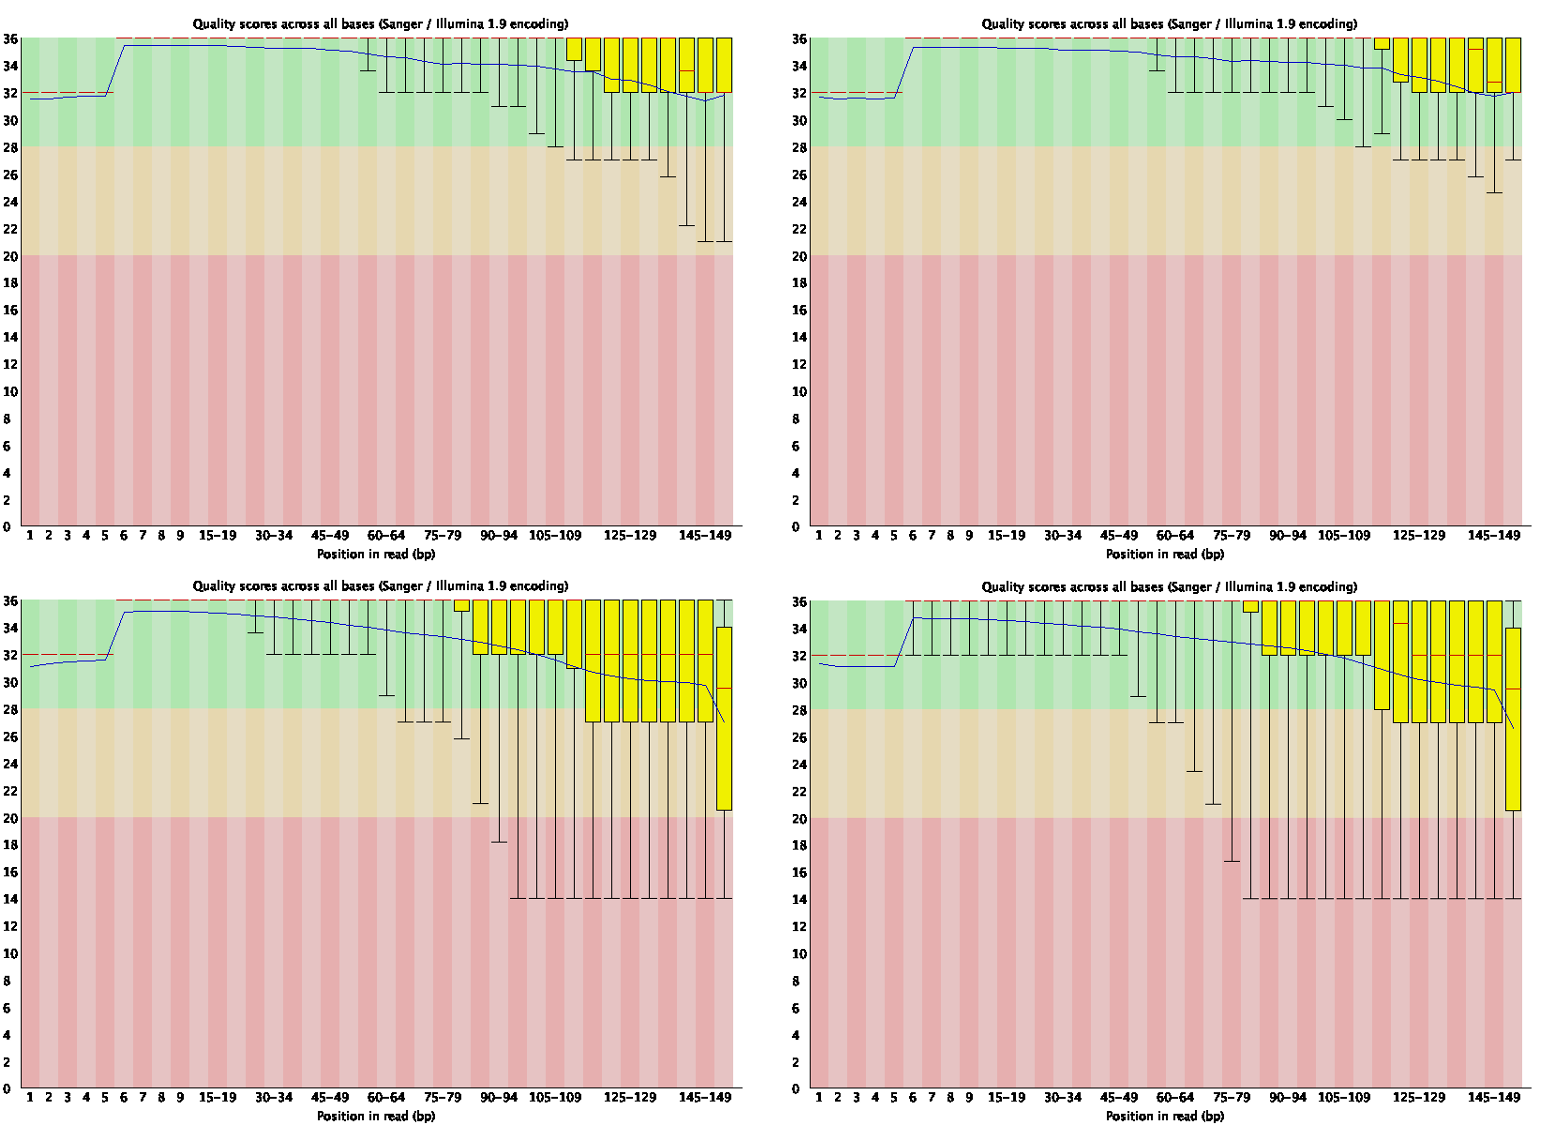
\includegraphics[scale=0.3]{fastqc/p1}
	\caption{Per base sequence quality score: [Top] AH [Bottom] CH. AH outperformed CH for both reads.
		Central red line shows the median value.
	Inter-quartile range 25-75\% (yellow box).
	Upper and lower whiskers represent the 10\% and 90\% points.
	Mean quality (blue line).
	}
	\label{fig:p1}
\end{center}
\end{figure}

\begin{figure}[h] \hspace*{0cm} 
\begin{center}
    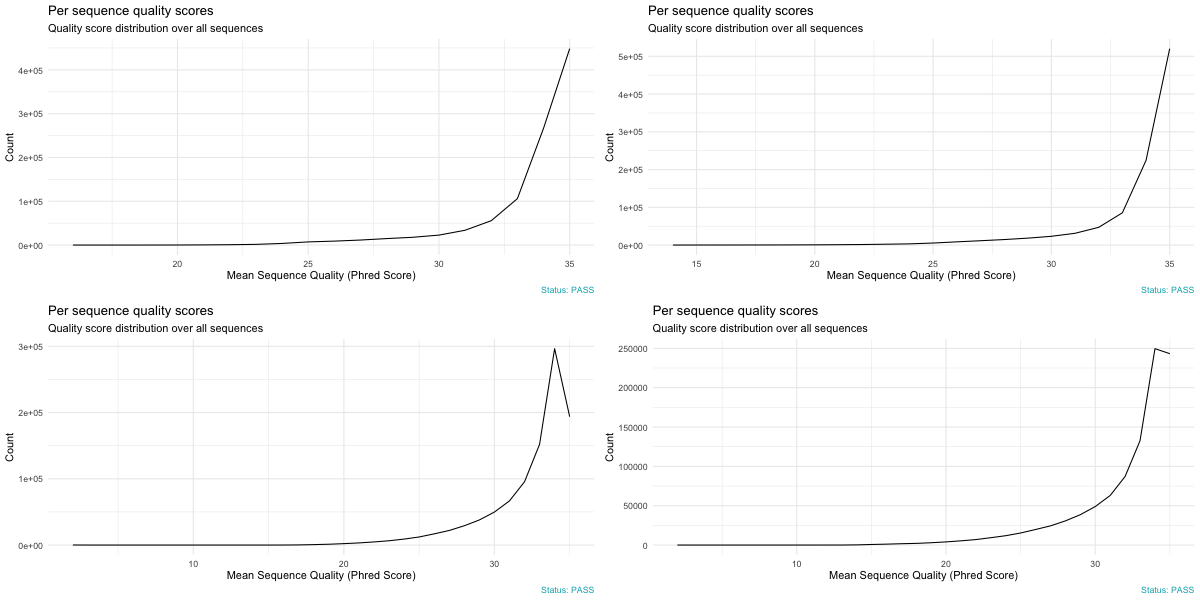
\includegraphics[scale=0.25]{fastqcr/p2}
	\caption{Per sequence quality score: [Top] AH [Bottom] CH. All samples performed sufficiently.  AH outperformed CH for both reads.
	Most frequently observed mean quality was above 30 for all samples; less than 0.2\% error rate.
	}
	\label{fig:p2}
\end{center}
\end{figure}

\begin{figure}[h] \hspace*{0cm} 
\begin{center}
    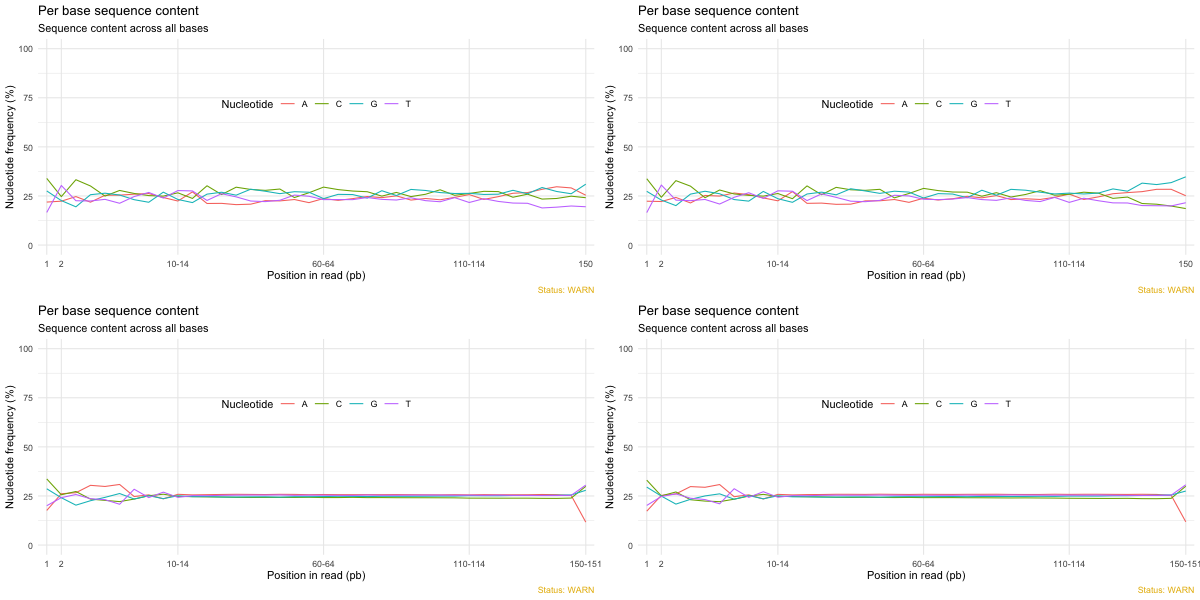
\includegraphics[scale=0.25]{fastqcr/p3}
	\caption{Per base sequence content: [Top] AH [Bottom] CH. \textit{Note}: The frequencies observed for CH are unexpected; additional background information is required for their interpretation.}
	\label{fig:p3}
\end{center}
\end{figure}

\begin{figure}[h] \hspace*{0cm} 
\begin{center}
    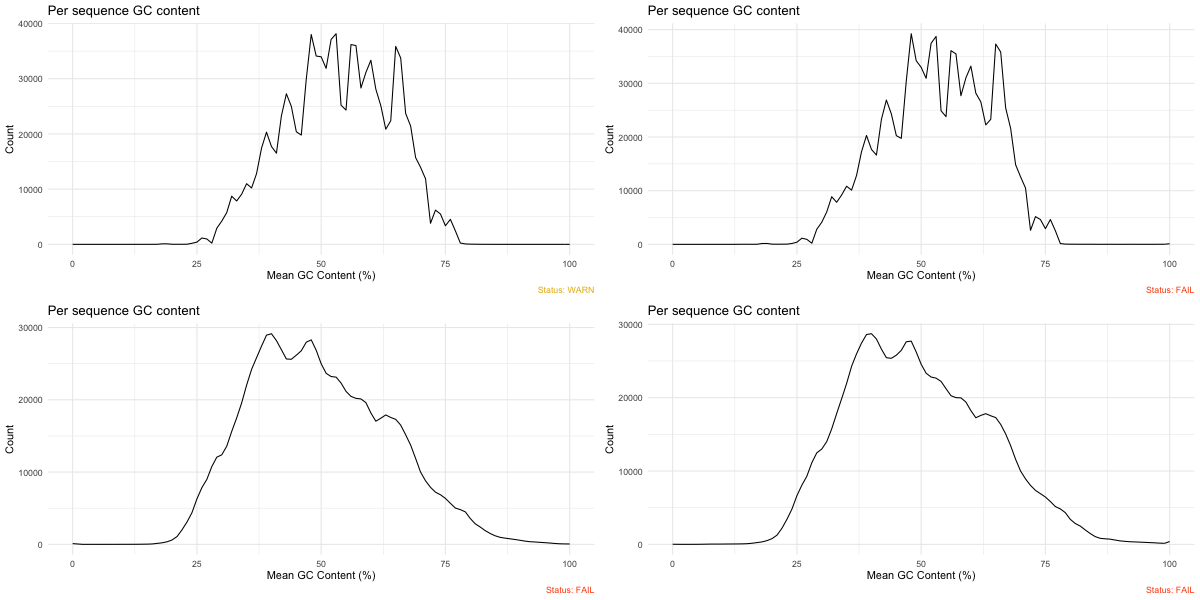
\includegraphics[scale=0.25]{fastqcr/p4}
	\caption{Per sequence GC content: [Top] AH [Bottom] CH.
	A normal distribution is expected for genomic DNA. However, targeted sequencing may produce difference distributions as seen here.}
	\label{fig:p4}
\end{center}
\end{figure}

\begin{figure}[h] \hspace*{0cm} 
\begin{center}
    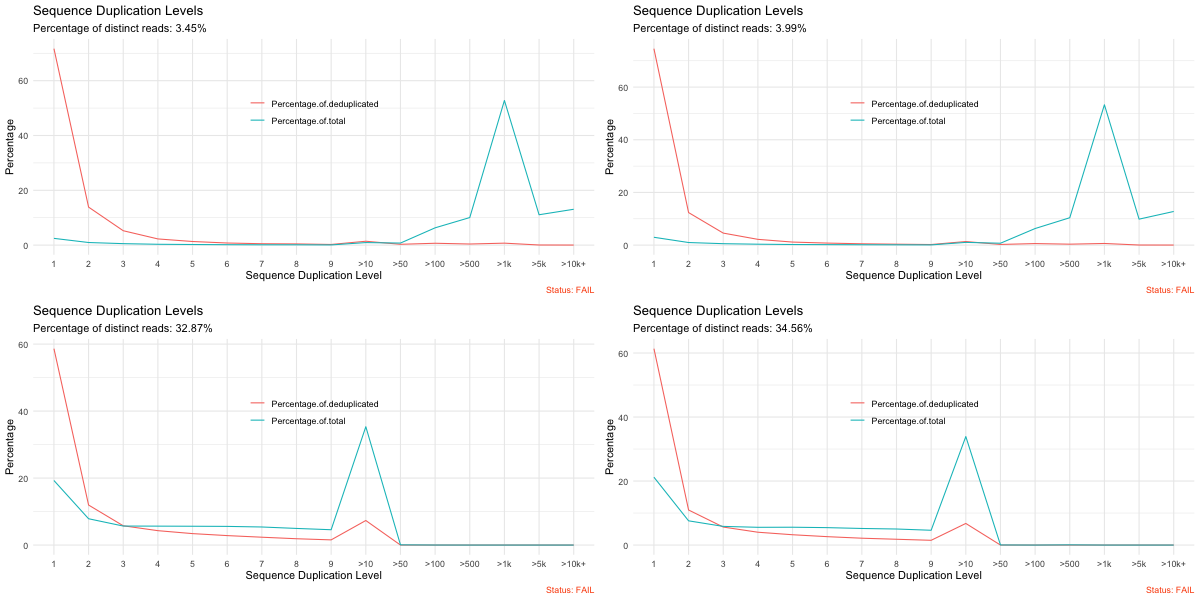
\includegraphics[scale=0.35]{fastqcr/p5}
	\caption{Sequence Duplication Levels:  [Top] AH [Bottom] CH.
	The plot shows the proportion of the library which is made up of sequences in each of the different duplication level bins. 
	The blue line shows the duplication level distribution for full sequence sets. 
	The red line shows de-duplicated sequences and the proportions shown are the proportions of the de-duplicated set which come from different duplication levels in the original data.
In a properly diverse library most sequences should fall into the far left of the plot in both the red and blue lines.
The fail status is due to non-unique sequences making up more than 50\% of the total, which is not a problem for targeted capture libraries.}
	\label{fig:p5}
\end{center}
\end{figure}

\begin{figure}[h] \hspace*{0cm} 
\begin{center}
    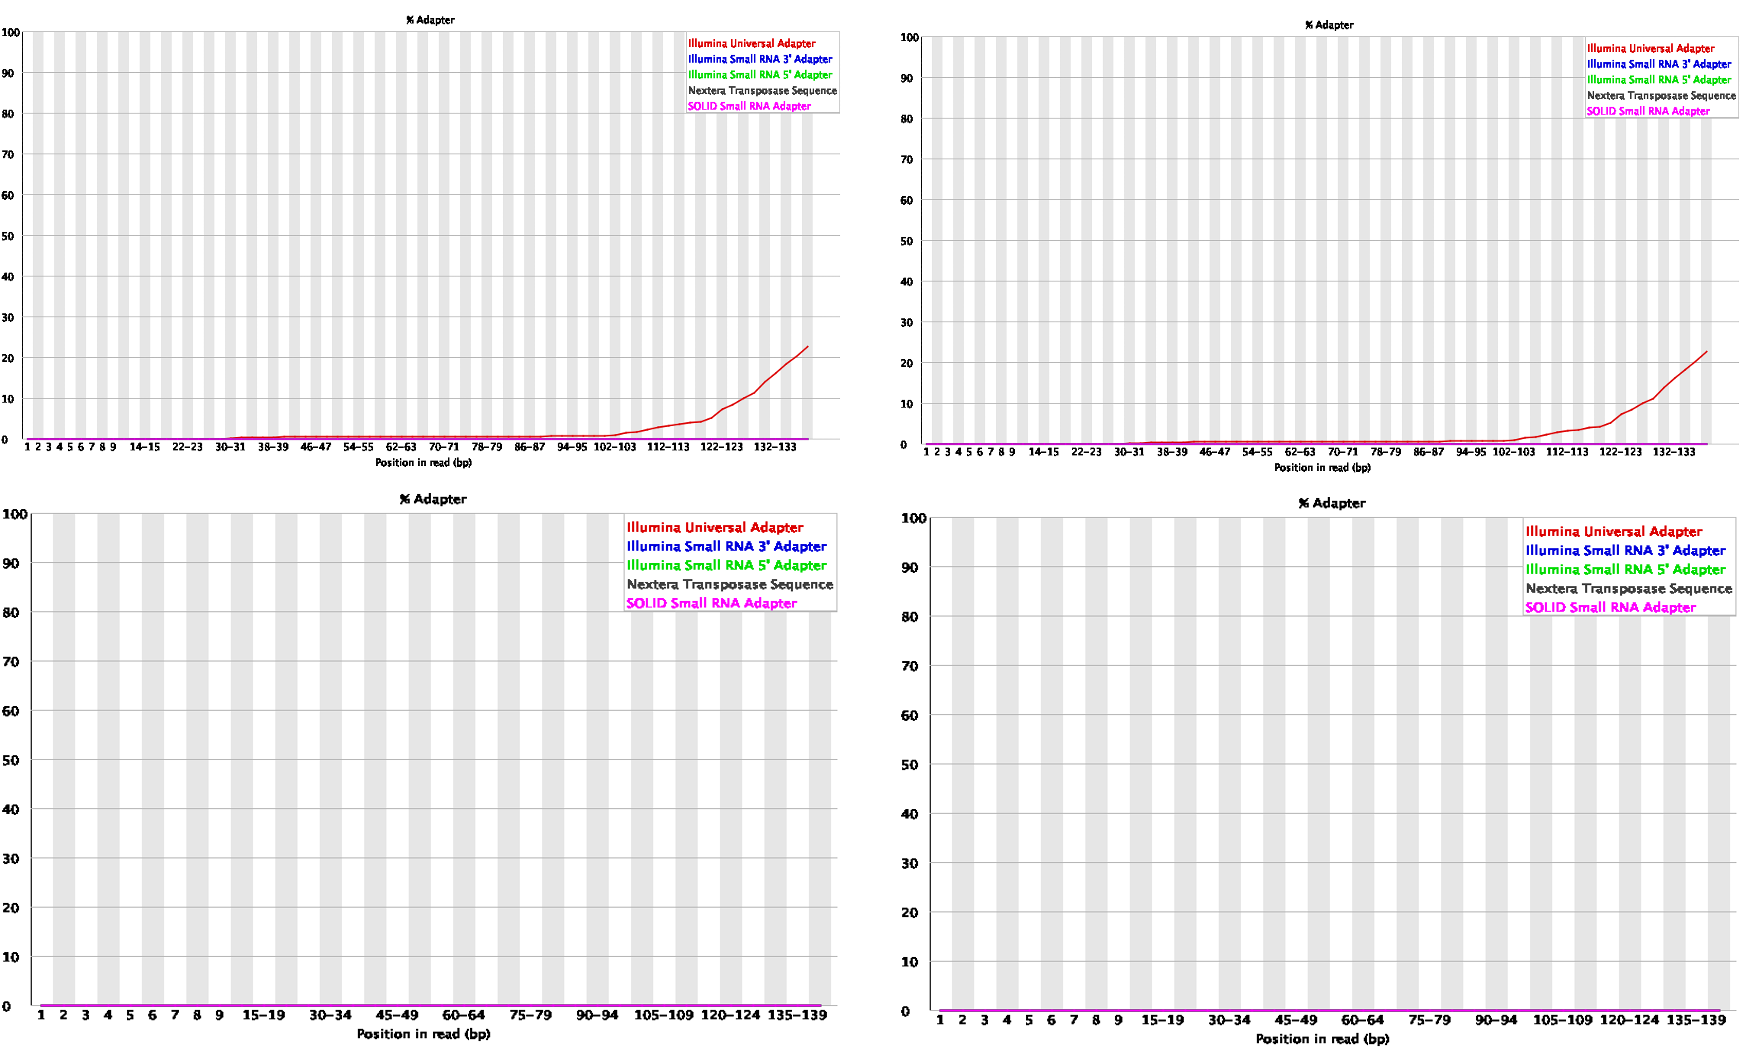
\includegraphics[scale=0.45]{fastqc/p6}
	\caption{Adapter content plot:  [Top] AH [Bottom] CH. Acumulative percentage count of the proportion of library which has seen each of the adapter sequences at each position. Adaptor sequence Illumina universal was found for AH, and no adaptor sequence was identified for CH. }
	\label{fig:p6}
\end{center}
\end{figure}

\clearpage

\subsection{Alignment data}
\label{align_data}
Fastq were trimmed using
\href{https://www.bioinformatics.babraham.ac.uk/projects/trim_galore/}{TrimGalore}.  
with the use of 
\href{ https://github.com/marcelm/cutadapt/}{cutadapt}.

Reads were aligned to GRCh37 using 
\href{http://bio-bwa.sourceforge.net}{BWA MEM} and converted to bam format with 
\href{http://www.htslib.org}{samtools}.

The aligment data was assessed using 
\begin{itemize}
\item \href{http://www.htslib.org}{samtools} flagstat: get mapping summary.
\item \href{http://www.htslib.org}{samtools} depth: read depth for at all positions of the reference genome, e.g. how many reads are overlapping the genomic position.
\item \href{http://qualimap.conesalab.org}{qualimap}: examines sequencing alignment data in SAM/BAM files according to the features of the mapped reads and provides an overall view of the data that helps to the detect biases in the sequencing and/or mapping of the data and eases decision-making for further analysis.
\end{itemize}

Qualimap full html report link:
\href{https://lawlessgenomics.com/pages/sophia/AH_S1_L001.sort_stats/qualimapReport.html}{sample AH}

Qualimap full html report link:
\href{https://lawlessgenomics.com/pages/sophia/CH_S2_L001.sort_stats/qualimapReport.html}{sample CH}

\begin{enumerate}
\item Samtools flagstat mapping summary shows alignment performance with GRCh37 for sorted reads, Table \ref{table:1}.\\
\item Mapping quality histogram indicate that AH performed better than CH, Figure \ref{fig:qualimap_map_qual_hist}.
\item Genome coverage histogram shows that AH produced a normal distribution of coverage depths while CH had an enrichment for some genomic regions, Figure \ref{fig:qualimap_gen_cov_hist}.
\item The duplication rate histograms are shown in Figure \ref{fig:qualimap_dup_hist}.
\item Genome coverage across GRCh37 shows a uniform distribution of reads for AH [Top], while CH [Bottom] has high depth in some regions with lower coverage in others, Figure \ref{fig:qualimap_gen_cov_ref}.
\end{enumerate}


\begin{center}	
\begin{table}[!b]
\caption{Samtools flagstat mapping summary. Alignment with GRCh37, sorted reads.}			
\begin{tabular}{ l l l } 				
 \hline				
CH	 & 	AH 	 & 	 \\
 \hline				
2011262	 & 	1999498	 & 	in total (QC-passed reads \& + QC-failed reads) \\ 
15710	 & 	612	 & 	secondary \\ 
0	 & 	0	 & 	supplementary \\ 
0	 & 	0	 & 	duplicates \\ 
2006501	 & 	1997929	 & 	mapped (99.76\% : N/A, 99.92\% : N/A) \\ 
1995552	 & 	1998886	 & 	paired in sequencing \\ 
997776	 & 	999443	 & 	read1 \\ 
997776	 & 	999443	 & 	read2 \\ 
1968314	 & 	1992738	 & 	properly paired (98.64\% : N/A, 99.69\% : N/A) \\ 
1986886	 & 	1996840	 & 	with itself and mate mapped \\ 
3905	 & 	477	 & 	singletons (0.20\% : N/A, 0.02\% : N/A) \\ 
14488	 & 	1612	 & 	with mate mapped to a different chr \\ 
8748	 & 	1426	 & 	with mate mapped to a different chr (mapQ>=5) \\ 
\hline				
\end{tabular}				
\label{table:1}
\end{table}
\end{center}	

\begin{figure}[ht] \hspace*{0cm} 
\begin{center}
    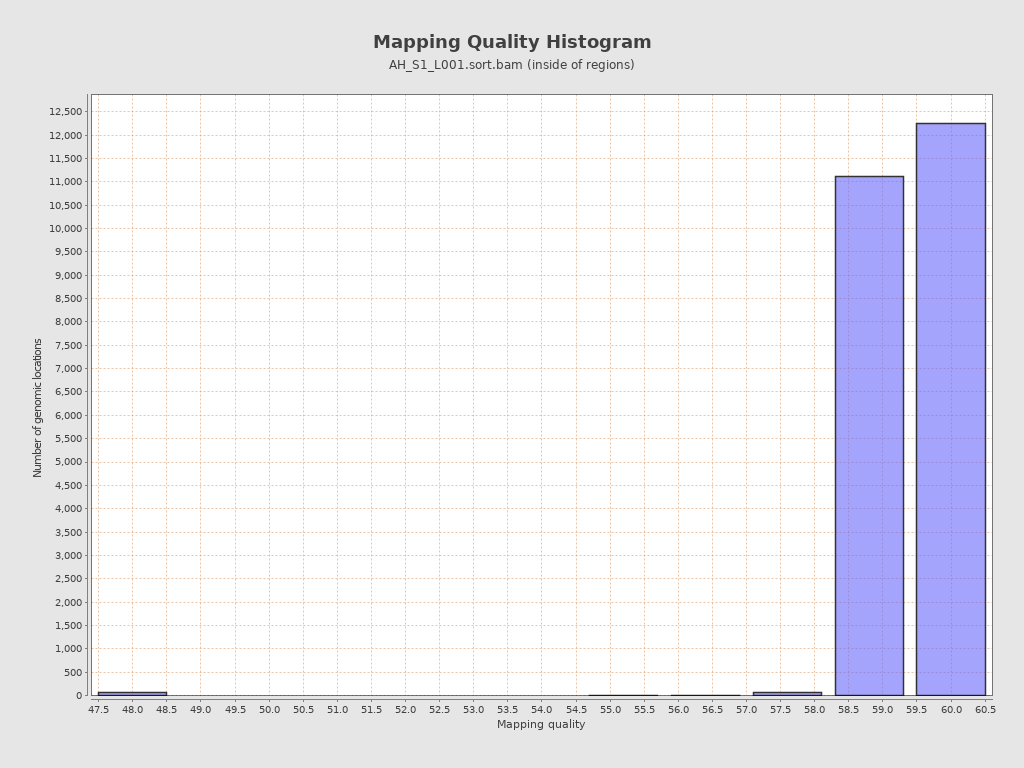
\includegraphics[scale=0.15]{qualimap/AH_S1_L001.sort_stats/images_qualimapReport/genome_mapping_quality_histogram}
        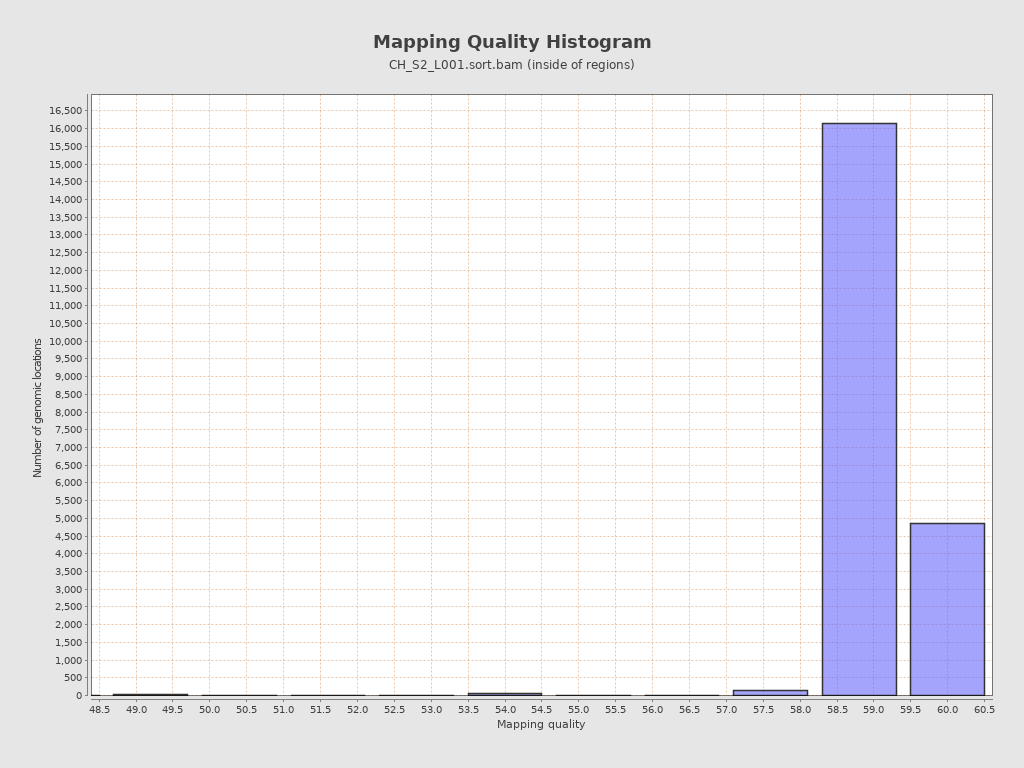
\includegraphics[scale=0.15]{qualimap/CH_S2_L001.sort_stats/images_qualimapReport/genome_mapping_quality_histogram}
	\caption{
	Mapping quality histogram (GRCh37). [Left] AH [Right] CH.
Histogram of the number of genomic locations having a given mapping quality. To construct the histogram mean mapping quality is computed at each genome position with non-zero coverage and collected. According to Specification of the SAM format the range for the mapping quality is [0-255].
	}
	\label{fig:qualimap_map_qual_hist}
\end{center}
\end{figure}

\begin{figure}[ht] \hspace*{0cm} 
\begin{center}
    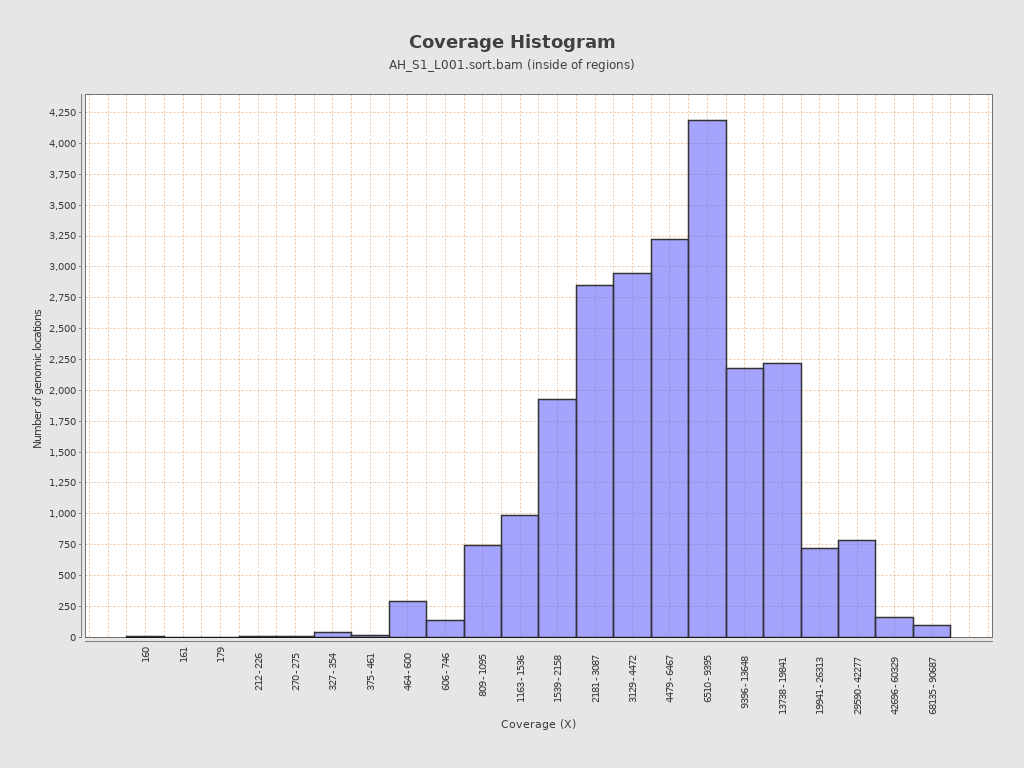
\includegraphics[scale=0.15]{qualimap/AH_S1_L001.sort_stats/images_qualimapReport/genome_coverage_histogram}
        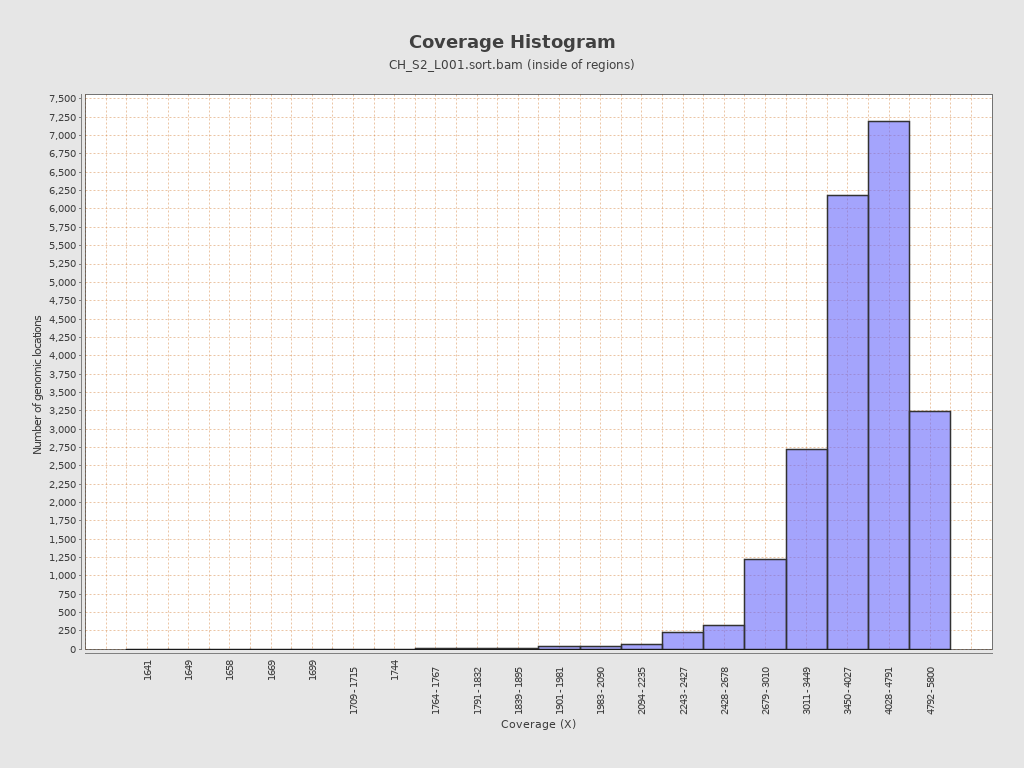
\includegraphics[scale=0.15]{qualimap/CH_S2_L001.sort_stats/images_qualimapReport/genome_coverage_histogram}
	\caption{
	Genome coverage histogram (GRCh37). [Left] AH [Right] CH.
	Histogram of the number of genomic locations having a given coverage rate. The bins of the x-axis are scaled by aggregating some coverage values in order to produce a representative histogram also in presence of the usual NGS peaks of coverage.
	}
	\label{fig:qualimap_gen_cov_hist}
\end{center}
\end{figure}

\begin{figure}[ht] \hspace*{0cm} 
\begin{center}
    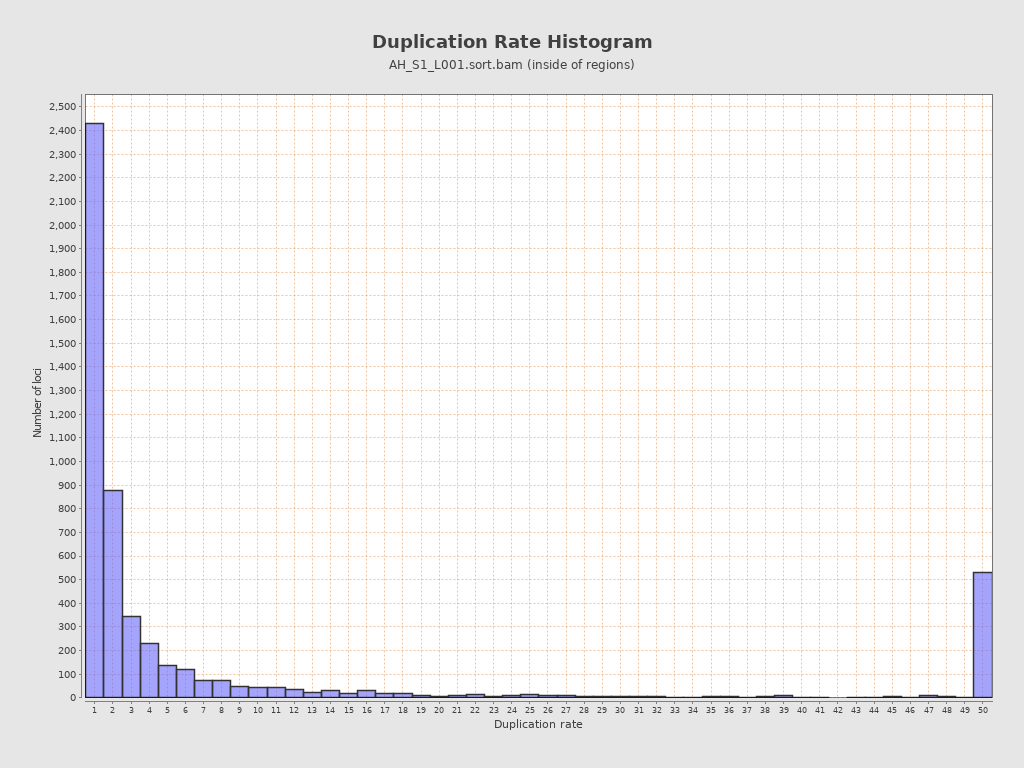
\includegraphics[scale=0.15]{qualimap/AH_S1_L001.sort_stats/images_qualimapReport/genome_uniq_read_starts_histogram}
        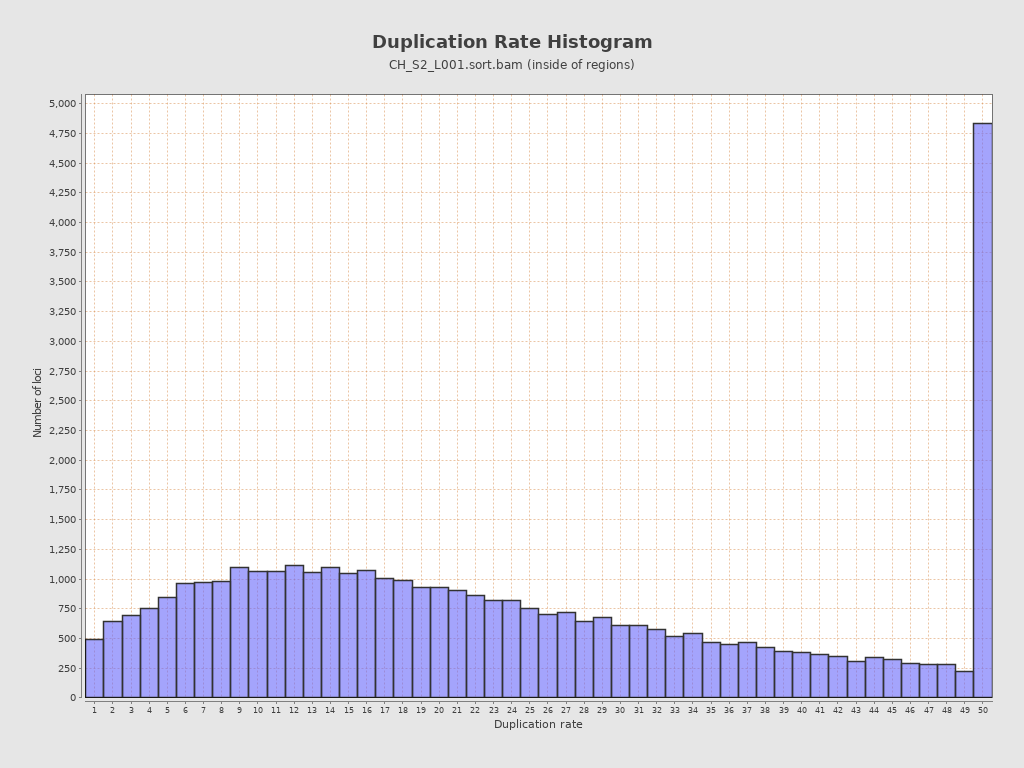
\includegraphics[scale=0.15]{qualimap/CH_S2_L001.sort_stats/images_qualimapReport/genome_uniq_read_starts_histogram}
	\caption{
	Duplication rate histogram (GRCh37). [Left] AH [Right] CH.
	This plot shows the distribution of duplicated read starts. Due to several factors (e.g. amount of starting material, sample preparation, etc) it is possible that the same fragments are sequenced several times. For some experiments where enrichment is used (e.g. ChIP-seq ) this is expected at some low rate. If most of the reads share the exact same genomic positions there is very likely an associated bias.
	}
	\label{fig:qualimap_dup_hist}
\end{center}
\end{figure}

\begin{figure}[ht] \hspace*{0cm} 
\begin{center}
    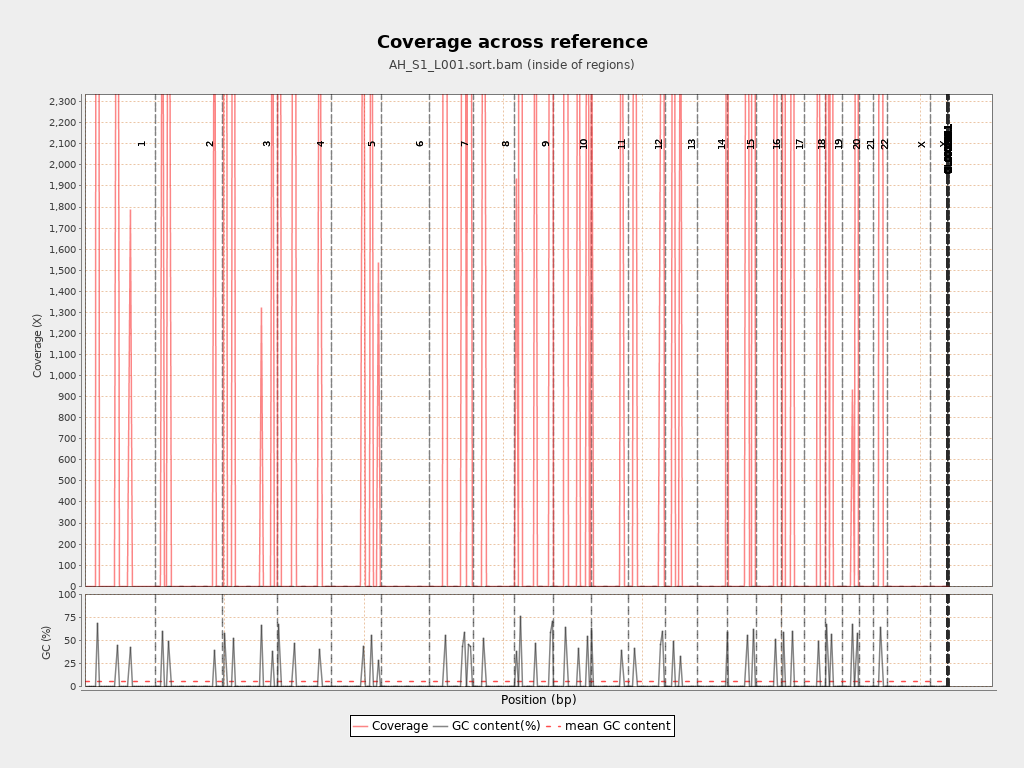
\includegraphics[scale=0.3]{qualimap/AH_S1_L001.sort_stats/images_qualimapReport/genome_coverage_across_reference}
        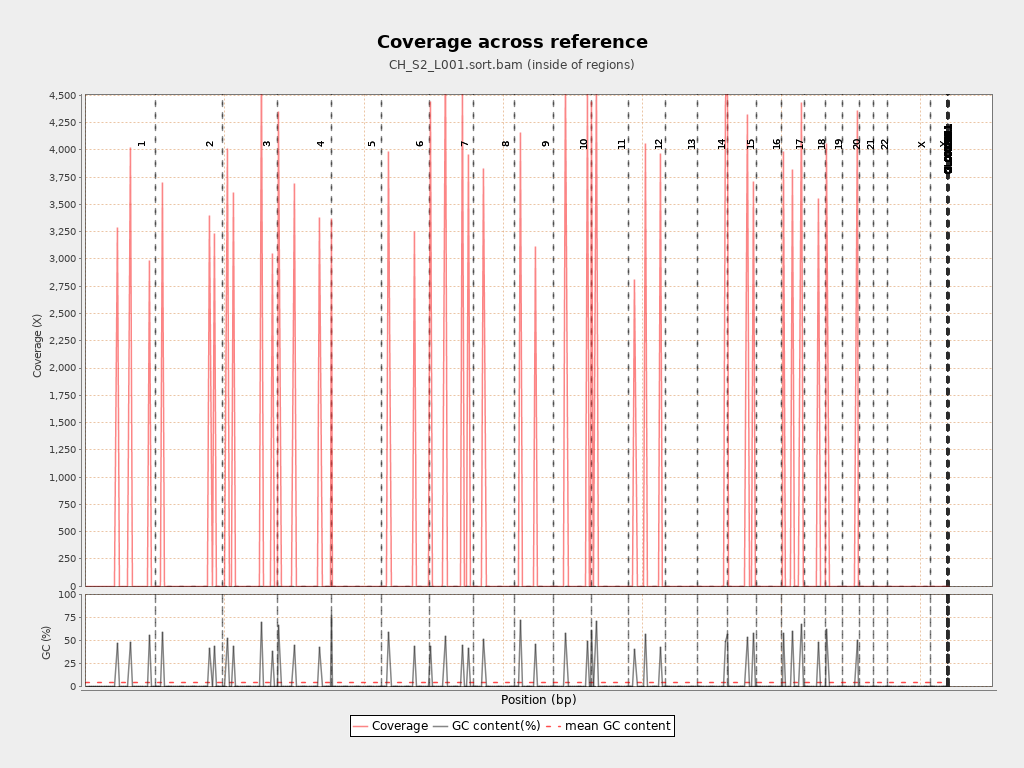
\includegraphics[scale=0.3]{qualimap/CH_S2_L001.sort_stats/images_qualimapReport/genome_coverage_across_reference}
	\caption{
	Genome coverage across reference (GRCh37). [Top] AH [Bottom] CH.
	Each plot consists of two figures. The upper figure provides the coverage distribution (red line) and coverage deviation across the reference sequence. The coverage is measured in X number of reads. The lower figure shows GC content across reference (black line) together with its average value (red dotted line).
	}
	\label{fig:qualimap_gen_cov_ref}
\end{center}
\end{figure}

\clearpage
\subsection{Target coding genes}
\label{coding}
To learn about what target regions are captured in this dataset, the coordinates (hg19) were annotated using Ensembl Biomart. The data was annotated using 
\href{http://grch37.ensembl.org/biomart/martview/3b67c8bb1f8be31e245e76a1b368fc8b}{grch37.ensembl.org/biomart}
dataset Ensembl Genes 105 (GRCh37.p13).
Output attributes queried for these regions: Gene stable ID, Transcript stable ID, Gene name, Gene start (bp), Gene end (bp), Chromosome/scaffold name, Gene \% GC content, HGNC symbol, and HGNC ID.
The gene symbols for each target list are shown in Table \ref{long}:
\begin{itemize}
	\item \href{https://lawlessgenomics.com/pages/sophia/target_info_biomart_simple.html}{Target coding genes table (html version).}
\end{itemize}

\begin{center}
\begin{longtable}{ l l l l l l l}
\caption{Targeted coding genes in GRCh37 present in for each method. \label{long}}\\
%
%\begin{tabular}{ l l l l l l l}
 \hline  
Chr & Start & End & Gene name & \% GC content & AH S1 & CH S2 \\
1 & 43803478 & 43818443 & MPL & 48.47 & Yes & No \\
1 & 115247090 & 115259515 & NRAS & 39 & Yes & Yes \\
1 & 162601163 & 162757190 & DDR2 & 40.47 & Yes & Yes \\
2 & 25455845 & 25565459 & DNMT3A & 53.5 & Yes & No \\
2 & 29415640 & 30144432 & ALK & 43.51 & Yes & Yes \\
2 & 47922669 & 48037240 & MSH6 & 44.65 & Yes & No \\
2 & 48016455 & 48132932 & FBXO11 & 39.46 & Yes & No \\
2 & 209100951 & 209130798 & IDH1 & 41.27 & Yes & Yes \\
2 & 212240446 & 213403565 & ERBB4 & 34.69 & Yes & Yes \\
3 & 10182692 & 10193904 & VHL & 47.55 & Yes & No \\
3 & 37034823 & 37107380 & MLH1 & 42.01 & Yes & No \\
3 & 41236328 & 41301587 & CTNNB1 & 39.91 & Yes & Yes \\
3 & 138663066 & 138665982 & FOXL2 & 64.62 & Yes & Yes \\
3 & 178865902 & 178957881 & PIK3CA & 35.78 & Yes & Yes \\
4 & 1795034 & 1810599 & FGFR3 & 65.82 & Yes & Yes \\
4 & 54243810 & 55161439 & FIP1L1 & 40.97 & Yes & Yes \\
4 & 55095264 & 55164414 & PDGFRA & 43.65 & Yes & Yes \\
4 & 55524085 & 55606881 & KIT & 40.87 & Yes & Yes \\
4 & 55919227 & 55958701 & RP11-530I17.1 & 40.25 & Yes & No \\
4 & 55944644 & 55991756 & KDR & 40.69 & Yes & No \\
4 & 153242410 & 153457253 & FBXW7 & 35.41 & Yes & Yes \\
4 & 153258807 & 153259250 & RP11-461L13.2 & 34.91 & Yes & No \\
5 & 112043195 & 112181936 & APC & 37.63 & Yes & No \\
5 & 112162910 & 112203279 & CTC-554D6.1 & 39.75 & Yes & No \\
5 & 149432854 & 149492935 & CSF1R & 48.1 & Yes & No \\
5 & 170814120 & 170838141 & NPM1 & 43.6 & Yes & No \\
7 & 55086714 & 55324313 & EGFR & 45.08 & Yes & Yes \\
7 & 55247443 & 55256627 & EGFR-AS1 & 50.41 & Yes & Yes \\
7 & 116312444 & 116438440 & MET & 39.03 & Yes & Yes \\
7 & 128828713 & 128853386 & SMO & 49.17 & Yes & No \\
7 & 128849616 & 128853386 & RP11-286H14.8 & 57.23 & Yes & No \\
7 & 140419127 & 140624564 & BRAF & 37.97 & Yes & Yes \\
7 & 148504475 & 148581413 & EZH2 & 39.21 & Yes & No \\
8 & 38268656 & 38326352 & FGFR1 & 50.55 & Yes & Yes \\
8 & 38279407 & 38283614 & RP11-350N15.4 & 50.78 & Yes & No \\
9 & 4985033 & 5128183 & JAK2 & 37.53 & Yes & No \\
9 & 5077163 & 5084580 & AL161450.1 & 34.29 & Yes & No \\
9 & 21802635 & 22032985 & RP11-145E5.5 & 40.29 & Yes & Yes \\
9 & 21967751 & 21995300 & CDKN2A & 41.19 & Yes & Yes \\
9 & 80331003 & 80646374 & GNAQ & 39.13 & Yes & Yes \\
9 & 133589333 & 133763062 & ABL1 & 44.47 & Yes & No \\
9 & 135766735 & 135820020 & TSC1 & 42.78 & Yes & No \\
9 & 139388896 & 139440314 & NOTCH1 & 63.39 & Yes & No \\
10 & 43572475 & 43625799 & RET & 55.73 & Yes & Yes \\
10 & 89622870 & 89731687 & PTEN & 35.77 & Yes & No \\
10 & 123237848 & 123357972 & FGFR2 & 45.41 & Yes & Yes \\
11 & 532242 & 537287 & HRAS & 69.01 & Yes & Yes \\
11 & 108093211 & 108239829 & ATM & 37.52 & Yes & No \\
11 & 108179246 & 108338258 & C11orf65 & 38.99 & Yes & No \\
12 & 25357723 & 25403870 & KRAS & 36.37 & Yes & Yes \\
12 & 112856155 & 112947717 & PTPN11 & 43.16 & Yes & Yes \\
12 & 121416346 & 121440315 & HNF1A & 52.2 & Yes & No \\
13 & 28577411 & 28674729 & FLT3 & 43.22 & Yes & No \\
13 & 48877887 & 49056122 & RB1 & 36.91 & Yes & No \\
14 & 105235686 & 105262088 & AKT1 & 64.08 & Yes & Yes \\
15 & 66679155 & 66784650 & MAP2K1 & 44.72 & Yes & Yes \\
15 & 66782086 & 66784447 & CTD-3185P2.1 & 44.37 & Yes & No \\
15 & 66782473 & 66790151 & SNAPC5 & 44.54 & Yes & No \\
15 & 90626277 & 90645736 & IDH2 & 52.54 & Yes & Yes \\
16 & 68771128 & 68869451 & CDH1 & 46.89 & Yes & No \\
17 & 7565097 & 7590856 & TP53 & 48.85 & Yes & Yes \\
17 & 37844167 & 37886679 & ERBB2 & 52.09 & Yes & Yes \\
18 & 48494389 & 48584514 & RP11-729L2.2 & 41.11 & Yes & No \\
18 & 48494410 & 48611415 & SMAD4 & 40.04 & Yes & Yes \\
19 & 1189406 & 1228428 & STK11 & 58.47 & Yes & No \\
19 & 3094408 & 3124002 & GNA11 & 61.66 & Yes & Yes \\
19 & 3118663 & 3119302 & AC005262.3 & 64.69 & Yes & Yes \\
19 & 17935589 & 17958880 & JAK3 & 54.93 & Yes & No \\
20 & 35973088 & 36034453 & SRC & 54.1 & Yes & No \\
20 & 57414773 & 57486247 & GNAS & 47.09 & Yes & Yes \\
22 & 24129150 & 24176703 & SMARCB1 & 50.77 & Yes & No \\
\hline
%\end{tabular}
\label{table:2}
\end{longtable}
\end{center}

\section{Conclusion}
\label{conclusion}
\textbf{[1]} Based on QC of fastq data (sec. \ref{fastq_data}), \textbf{AH S1 outperformed CH S2}.
\textbf{[2]} Based on QC after alignment to reference genome GRCh37 (sec. \ref{align_data}), 
\textbf{AH S1 outperformed CH S2.} 
However, it should be noted that non-uniform coverage favouring a subset of genes might be preferable
in some circumstances;  additional information on study design required.
\textbf{[3]} Based on coverage for coding sequences within targeted regions (sec. \ref{coding}), \textbf{AH S1 outperformed CH S2}. 
However, additional information on study design required for confirmation.\\

\textbf{Summary}: AH S1 outperformed CH S2 on all tests.

\section{Colophon}
% Why are are hyperlinks so complex? 
% To minimise manual editing, figures that are used within this document are synced into the images directory. 
% However, the original parent directory structures are retained to mirror the data repository.
This document style is derived from the web design for SOPHiA GENETICS, using fonts  Source Sans Pro (light, regular, and italic).
Font colors are set as ``sophiablue'' \#0A2E4A and  ``sophiapink'' \#E32A5C.
Writing was done using LaTeX and html pages are hosted on 
\href{https://lawlessgenomics.com}{https://lawlessgenomics.com}.
For contact:  \href{https://lawlessgenomics.com/resume/pdf/Dylan_Lawless.pdf}{see here}.
\bibliographystyle{unsrtnat}
\bibliography{references}

\end{document}


